\subsection{Electronics}
The custom rotator is controlled by a Raspberry Pi, extended by a custom Raspberry Pi hat. The hat provides functionality to read the safety switches, communicate to two independent magnetic encoders, drive both motors, and monitor the motors speed with a quadrature encoder. The Hat also features an EEPROM, which is specified by the Raspberry Pi foundation, to call it an 'official' pi hat. The pi and both motors are powered through an of the shelf power over Ethernet (POE) adapter.

\subsubsection{choice of electronics}
We had a working prototype within the first couple of weeks, which enabled us to test lots of features early on. In the beginning, we needed three cables to power the Raspberry Pi, the motors, as well as to provide a data cable for communication. The power over Ethernet adapter allowed us to only have one cable and simplify the design.
To move away from our original breadboard design connected to some of the shelves components, we also designed our Raspberry Pi hat.


\subsubsection{how to connect, pinout}

The motors we used had a standard female header with a 2.54 mm pitch. We decided to stick with these connectors and used a standard female header for all connections. These female headers can be plugged into the matching male header on the PCB. All Connectors match the same side as the USB/ Ethernet etc. connections on the Raspberry Pi. That's to make the overall cable management simpler and cleaner.
The connectors are stacked on top. The board can drive two motors. One motor can be plugged in to the upper row, and the other on the lower row. The three switches are stacked on each other in the same way.

\begin{figure}[H]
	\centering
	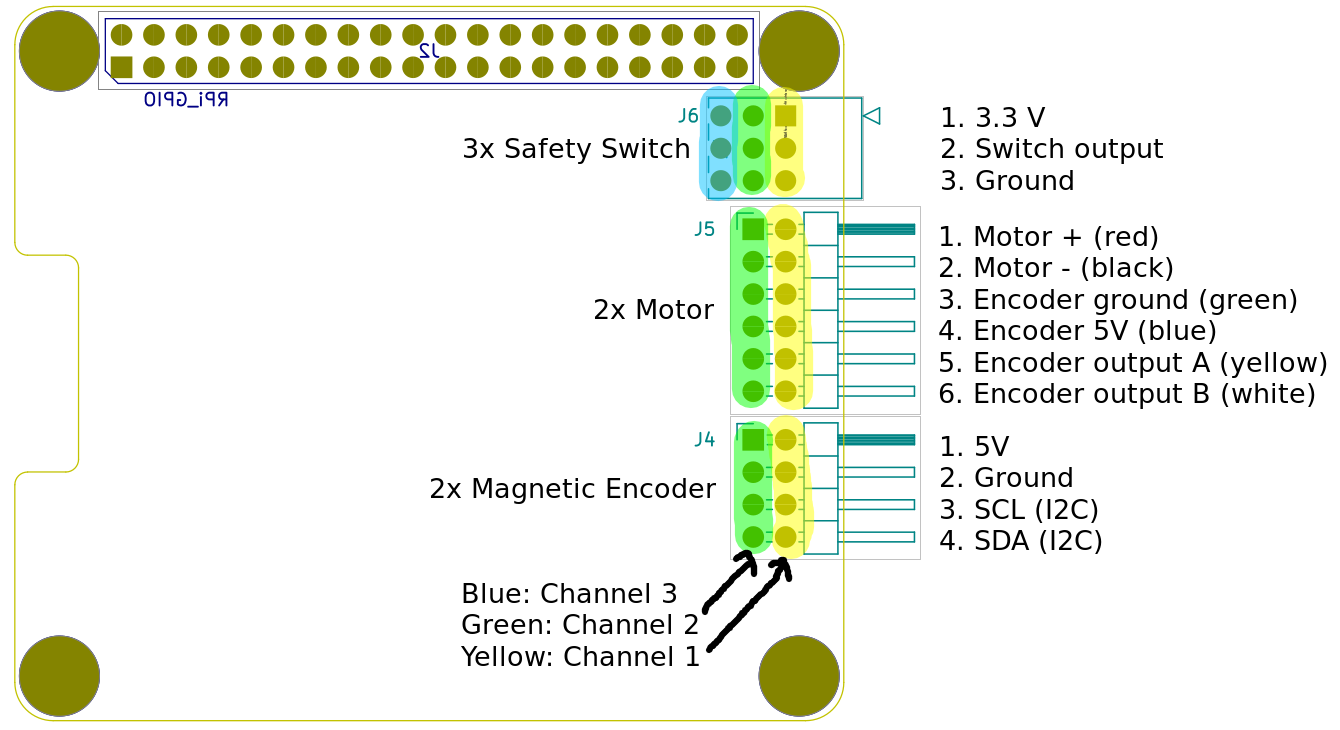
\includegraphics[scale=0.2]{../art/PCB Pinout.png}
	\caption{Raspberry Pi hat pinout}
\end{figure}

\subsubsection{Electronic Design}

The Raspberry Pi controls all components on the pi hat. The h-bridge, that drives the Motors, is powered externally with a 12V power source from the power over Ethernet hat. The encoder from the motors are connected through a level shifter to the Raspberry Pi. The Switches, on the other hand, are connected to the pi directly. The magnetic encoder both use the same i2c protocol. Unfortunately, they have the same address, which can't be changed. If both encoder, are put on the same i2c bus, the pi couldn't differentiate between those two, because they use the same address. The board features therefore an i2c multiplexer, which can select on encoder at a time. The i2c multiplexer is controlled by the same i2c bus. This reduces complexity on the board, but increases complexity in the code. The following diagram shows the structure.

\begin{figure}[H]
	\centering
	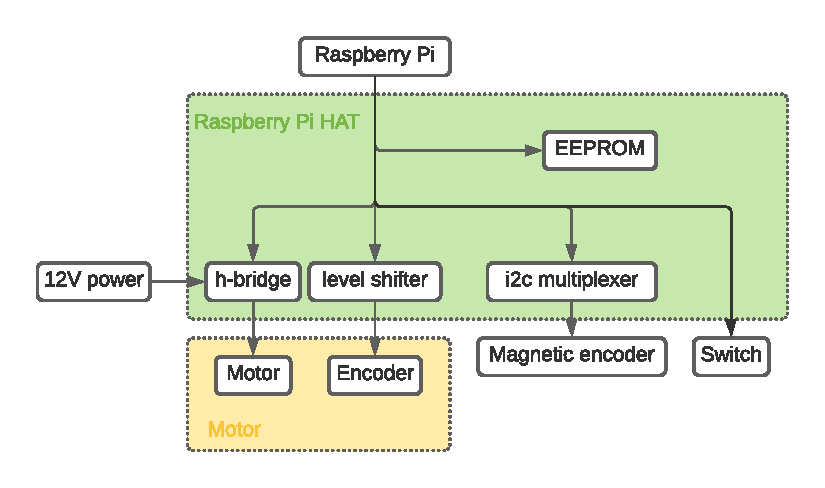
\includegraphics[width=\linewidth]{../art/PCB Block diagram.pdf}
	\caption{Raspberry Pi HAT block diagram}
\end{figure}


\subsubsection{development and fabrication}


We used KiCad to design the PCB. To solder the SMD components (IC's, resistors, capacitors etc.) of the PCB, we used a soldering a reflow oven. The remaining THT components (pin headers etc.) were soldered manually. The schematic, the final pcb, as well as the manufactureing process in the reflow oven are listed in the appendix.
